% Etapa 1 do enunciado: modelagem dos 5 objetos.
% Fonte no código: primitives.py, modeling.py
% Função que retorna o sólido: modeling.criar_solido. Figuras: visualizar_objetos.py (salvas pelo botão de salvar da janela).
\subsection{Modelagem dos objetos}\label{sec:modelagem}

Os cinco objetos foram modelados cada um no seu sistema de coordenadas, apoiados em $y = 0$ e
centrados no eixo $y$. Só o haltere fica deitado, ao longo do eixo $x$.

Cada objeto é uma função $F(x, y, z)$ que vale menos que zero dentro do objeto, zero na superfície e
mais que zero fora. Formas simples (cilindro, cone, esfera, caixa e toro) são combinadas: a união é
o mínimo entre as funções e a subtração é $\max(A, -B)$, usada para deixar a lixeira oca. O
algoritmo \textit{Marching Cubes} \cite{lorensen1987}, da biblioteca scikit-image
\cite{vanderwalt2014}, recebe $F$ em uma grade de 80 pontos por eixo e devolve os triângulos de
$F = 0$.

A função \texttt{criar\_solido} devolve vértices, faces, arestas, normais das faces, normais dos
vértices e cor, tudo em coordenadas do objeto. As normais apontam para fora. Em todos os objetos, a
malha satisfaz $V - A + F = 2$, o que indica superfície fechada e sem buracos. A
Figura~\ref{fig:objetos} mostra os objetos com os eixos e as normais de algumas faces (setas
pretas), em uma grade de 50 pontos por eixo, mais leve para exibir. A cena usa 80 pontos.

\begin{figure}[H]
  \centering
  \caption{Objetos no sistema de coordenadas do objeto}\label{fig:objetos}
  \begin{subfigure}{0.31\textwidth}
    \centering
    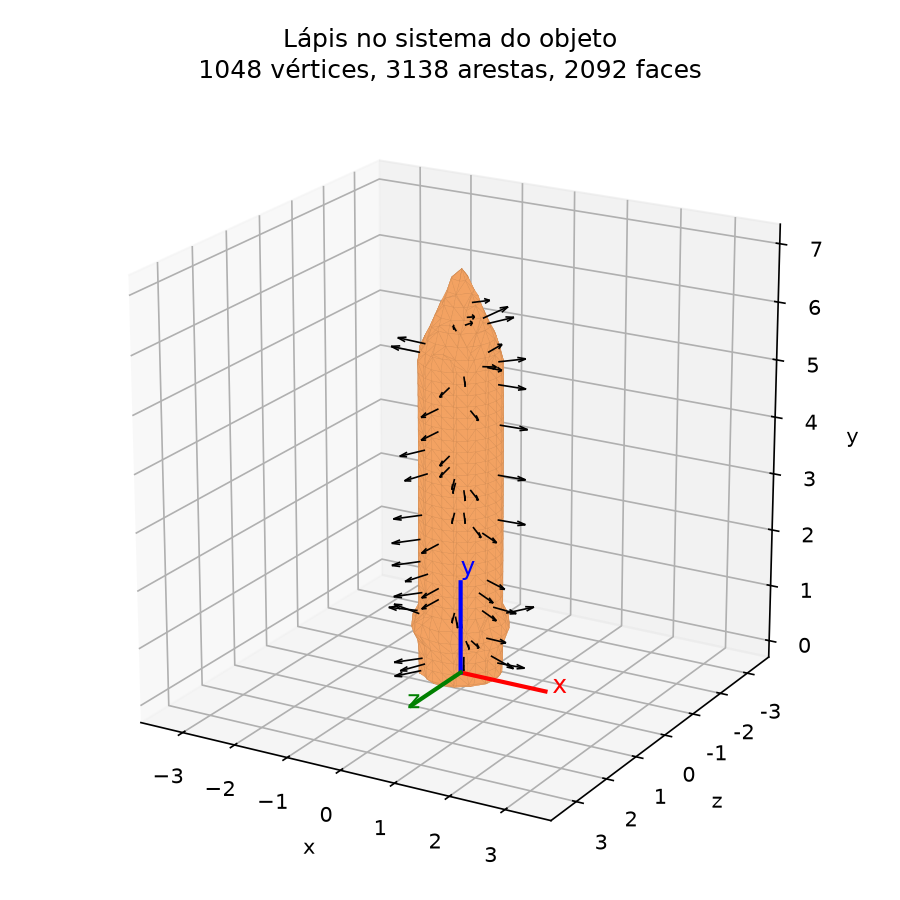
\includegraphics[width=\textwidth]{03-desenvolvimento/01-modelagem/lapis.png}
    \caption{Lápis}
  \end{subfigure}\hfill
  \begin{subfigure}{0.31\textwidth}
    \centering
    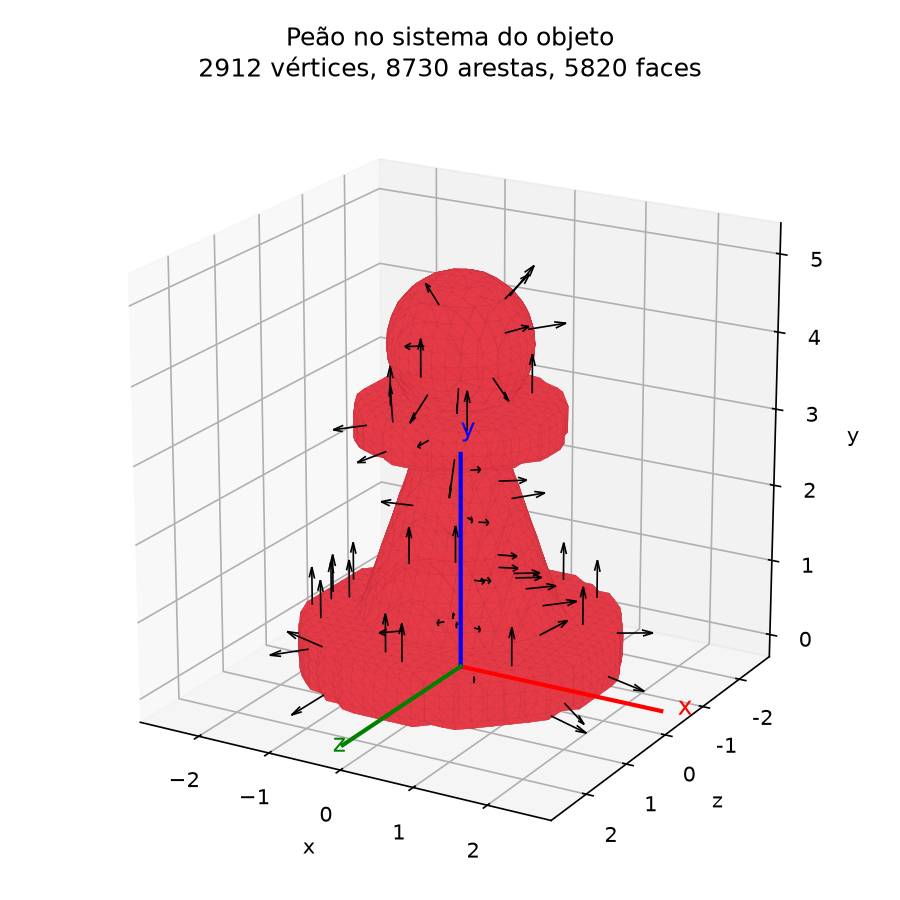
\includegraphics[width=\textwidth]{03-desenvolvimento/01-modelagem/peao.png}
    \caption{Peão}
  \end{subfigure}\hfill
  \begin{subfigure}{0.31\textwidth}
    \centering
    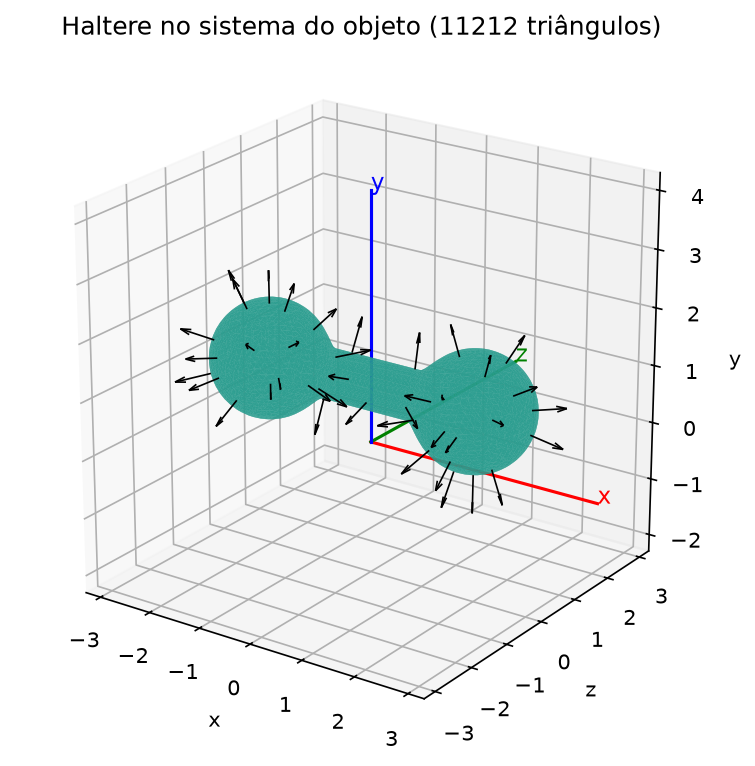
\includegraphics[width=\textwidth]{03-desenvolvimento/01-modelagem/haltere.png}
    \caption{Haltere}
  \end{subfigure}

  \vspace{6pt}
  \begin{subfigure}{0.31\textwidth}
    \centering
    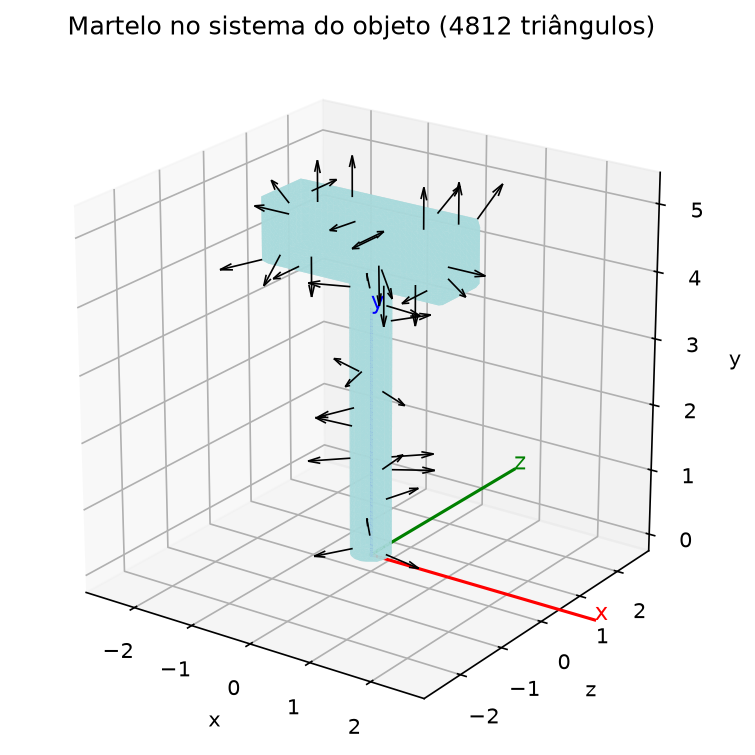
\includegraphics[width=\textwidth]{03-desenvolvimento/01-modelagem/martelo.png}
    \caption{Martelo}
  \end{subfigure}\hspace{0.04\textwidth}
  \begin{subfigure}{0.31\textwidth}
    \centering
    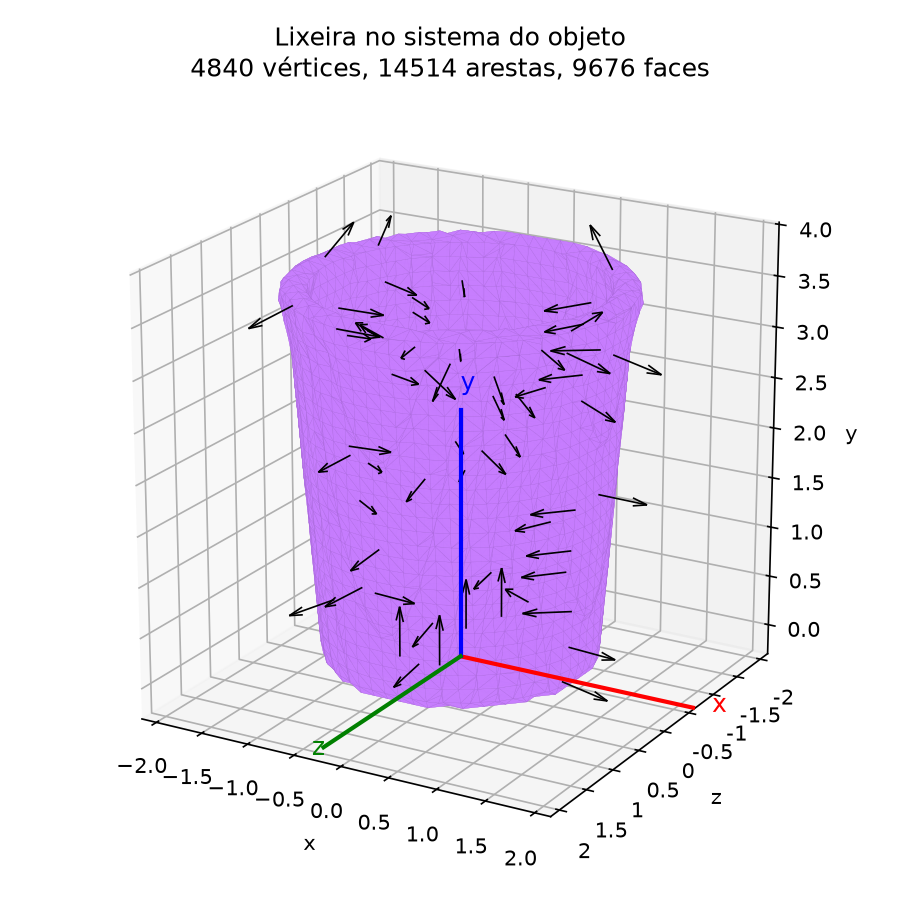
\includegraphics[width=\textwidth]{03-desenvolvimento/01-modelagem/lixeira.png}
    \caption{Lixeira}
  \end{subfigure}
  \fonte{Autoria própria (2026)}
\end{figure}
